

\begin{document}

\title{Wayside Controller User Manual}
\author{Written by: Max Reno}
\date{}

\maketitle

\section{Wayside Controller}

\subsection{UI Layout}

\begin{figure}[h!]
	\center
	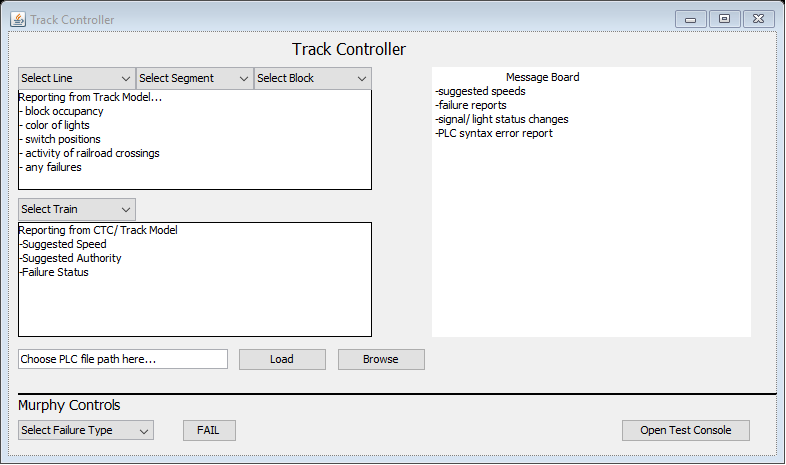
\includegraphics[width=16cm]{trackcontroller_gui}
	\caption{Graphical User Interface for the track controller.}
\end{figures}


\subsection{UI Buttons and Actions}

	\subsubsection{Block Selection}
		\begin{itemize}
			\item Series of Dropdowns - used to select appropiate line/segment/block
			\item Text Display - displays information such as block occupancy, switch status, light color and status, activity of railroad crossings and any failures that it may report to the CTC.
		\end{itemize}
	\subsubsection{Train Selection}
		\begin{itemize}
			\item Text Display - reports on the suggested speed and authority as received from the CTC as well as any failures which would need to be reported back the CTC/track model.
		\end{itemize}
	\subsubsection{File Browser/Loader}
		\begin{itemize}
			\item Text Field - can input file path here directly or use the browse option as follows.
			\item Load Button - Load button – once file is chosen, pressing load will load the given PLC file and run it accordingly.
			\item Browse button – this will propagate a pop up window which will allow the user to browse through their computer to find the appropriate file that they wish to load.
		\end{itemize}
	\subsubsection{Message Board}
		\begin{itemize}
			\item Text display – this field will display any info that doesn’t apply to the two other fields such as: debugging PLC or changing failures statuses.
		\end{itemize}
	\subsubsection{Murphy}
		\begin{itemize}
			\item Dropdown – select the type of failure that the user wishes to instantiate.
			\item Fail button – instantiates the given type of failure.
			\item Open Test Console button – pushing this button opens a pop up window of the testing console as follows.
		\end{itemize}


\subsection{UI Testing Layout}

\begin{figure}
	\center
	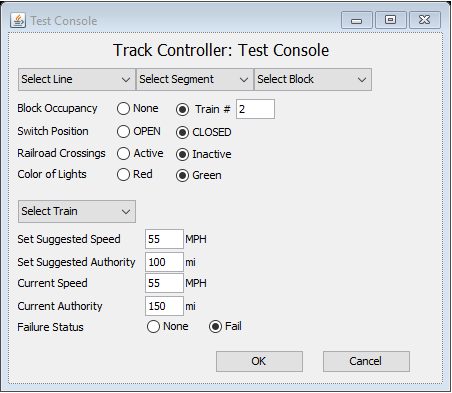
\includegraphics[width=12cm]{trackcontrollertestconsole_gui}
	\caption{Graphical user Interface for the test console of the wayside controller.}
\end{figure}


\subsection{UI Buttons and Actions} 

	\subsubsection{Block Selection}
		\begin{itemize}
			\item Series of Dropdowns – used to select appropriate line/segment/block.
		\end{itemize}

	\subsubsection{Block Testing Situations}
		\begin{itemize}
			\item Series of Radio Buttons -
				\begin{itemize}
					\item Block Occupancy – either clears the block of all trains or adds a given train into this block in order to report on it.
					\item Switch Position – closed will keep it in the same position, while open will change it.
					\item Railroad Crossings – triggers them to be on or off should a given block have them.
					\item Color of lights – triggers the lights to either color in order to report on it.
				\end{itemize}
		\end{itemize}

	\subsubsection{Train Testing Situations}
		\begin{itemize}
			\item Series of Text Inputs – allows user to give inputs as if the track/CTC didn’t exist in order to test it on its own.
		\end{itemize}
	\subsubsection{Ok/Cancel Buttons – passes the information chosen here onto the original UI to show testing.}

\end{document}
	






